\documentclass[mathserif]{beamer}

\usetheme[secheader]{Madrid}
\setbeamercovered{transparent=50}

\usepackage{tikz}
%\usetikzlibrary{trees}
\usepackage{url}
\usepackage{graphicx}

\usepackage{pygments}
\usepackage{graphicx}

\providecommand{\code}[1]{{\texttt{\scriptsize{#1}}}}
\providecommand{\inputcode}[1]{
  \begin{block}{}
    \scriptsize{\input{#1}}
  \end{block}
}

\title[OO Design]{Object Oriented Design for Physical Simulation}
\author{Joel Berger}
\institute[UIC]{University of Illinois at Chicago}
\date{October 3, 2012}

\begin{document}

\begin{frame}
  \maketitle
\end{frame}

\begin{frame}{Outline}
  \tableofcontents
\end{frame}

\AtBeginSection{
  \begin{frame}{Outline}
    \tableofcontents[currentsection]
  \end{frame}
}

\section{Programming Styles}

\begin{frame}{Programming Styles}
  There are several common programming styles
  \begin{itemize}
    \item Procedural
    \item Functional
    \item Object Oriented
  \end{itemize}
\end{frame}

\begin{frame}{Procedural Programming}
  \begin{block}{Procedural Programming}
    Functions are like tasks, acting on external variables
  \end{block}
  \begin{columns}
    \begin{column}{0.49\linewidth}
      \uncover<2->{\inputcode{styles/procedural}}
    \end{column}
    \begin{column}{0.49\linewidth}
      \begin{itemize}
        \item[$+$]<3-> Code is simple (steps)
        \item[$-$]<4-> Code is not reusable
        \item[$-$]<5-> Depends on global variables
        \item[$-$]<6-> Procedures are tied to certain variables
      \end{itemize}
    \end{column}
  \end{columns}
\end{frame}

\begin{frame}{Functional Programming}
  \begin{block}{Functional Programming}
    Functions are like transforms, taking inputs and returning results
  \end{block}
  \begin{columns}
    \begin{column}{0.49\linewidth}
      \uncover<2->{\inputcode{styles/functional}}
    \end{column}
    \begin{column}{0.49\linewidth}
      \begin{itemize}
        \item[$+$]<3-> Code is reusable
        \item[$-$]<4-> Lots of data to track
        \item[$-$]<5-> Must take care to manipulate the right data
      \end{itemize}
    \end{column}
  \end{columns}
\end{frame}

\begin{frame}{Object Oriented Programming}
  \begin{block}{Object Oriented Programming}
    Objects have internal data, methods (functions) act on inputs and that data
  \end{block}
  \visible<2->{\inputcode{styles/objective}}
\end{frame}

\section{Object Oriented Programming}

\begin{frame}{Class Structure}
  A \alert{Class} is a particular type of object. Classes have
  \begin{itemize}
    \item \alert{Attributes} - internal data
    \item \alert{Methods} - functions tied to the class/object
    \item \alert{Accessor Methods} - special functions for accessing the attribute data
  \end{itemize}

  An individual object is said to be an \alert{Instance} of a certain class
\end{frame}

\begin{frame}{Subclasses}
  A \alert{Subclass} is a class which redefines or adds on to a \alert{Parent} class. 

  \inputcode{examples/student}
\end{frame}

\section{Physical Simulations}

\begin{frame}{Back to Physics}
  Ok this has been some good C.S. info, but where is the Physics?
\end{frame}

\subsection{A Simple OO-DE Example}

\begin{frame}{Physical Classes}
  \inputcode{code/class0}
\end{frame}

\begin{frame}{The Solver: Attributes}
  \inputcode{code/class1}
\end{frame}

\begin{frame}{The Solver: Methods}
  \inputcode{code/class2}
\end{frame}

\begin{frame}{The Script}
  \begin{columns}
    \begin{column}{0.49\linewidth}
      \inputcode{code/example1}
    \end{column}
    \begin{column}{0.49\linewidth}
      \inputcode{code/example2}
      \vspace{4mm}
      \centering
      \visible<2->{
        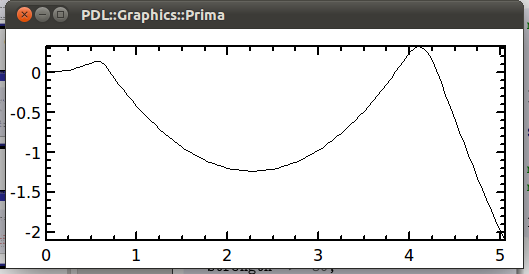
\includegraphics[width=0.8\linewidth]{example.png}
      }
    \end{column}
  \end{columns}
\end{frame}

\end{document}
